\chapter{Introduction}

%\label{sec:introduction}

Access control is one of the most fundamental and widely used
security mechanisms, especially in web applications. It controls
which principals such as users or processes have access to which
resources in a system. To facilitate managing and maintaining access
control, access control policies are increasingly written in
specification languages such as XACML~\cite{oasis05:xacml} and
Ponder~\cite{damianou01:ponder}. Whenever a principal requests
access to a resource, that request is passed to a software component
called a \Intro{Policy Decision Point} (PDP). A PDP evaluates the
request against the specified access control policies, and permits
or denies the request accordingly.

Assuring the correctness of policy specifications is becoming an
important and yet challenging task, especially as access control
policies become more complex and are used to manage a large amount
of sensitive information organized into sophisticated structures.
Identifying discrepancies between policy specifications and their
intended function is crucial because correct implementation and
enforcement of policies by applications is based on the premise
that the policy specifications are correct. As a result, policy
specifications must undergo rigorous verification and validation
through systematic testing to ensure the policy specifications
truly encapsulate the desires of the policy authors.

Software testing is an important and practical technique to
efficiently detect errors in complex software systems. Errors in
policy specifications may also be discovered by leveraging existing
techniques for software testing. Figure~\ref{fig:policy-test}
illustrates the analogy between software testing and policy testing.
In policy testing, test inputs are access requests and test outputs
are access responses. The execution of a test input occurs as a
request is evaluated by the PDP against the access control policy
under test. Policy authors can inspect request-response pairs to
check whether they are as expected. As with software verification,
formal policy verification and testing techniques are complementary
means to achieve the same goal.

Mutation testing~\cite{demillo78:hints} has historically been
applied to general-purpose programming languages in measuring the
quality of a test suite. In this paper, we propose a fault model for
access control policies. We present a new framework that implements
this fault model to facilitate automated mutation testing of access
control policies. In the framework, we define a set of new mutation
operators for XACML policies based on the fault model. We also
develop a new tool that automatically seeds a policy under test with
faults by applying these mutation operators, thereby producing
numerous mutant policies. We leverage a change-impact analysis tool
to detect equivalent mutants among generated mutants. We determine
whether a mutant policy is killed by a request by comparing the
responses for the request based on the original policy and mutant
policy. Our framework can be applied on XACML policies together with
previous tools we have developed for test generation, test
selection, and structural coverage measurement for access control
policies~\cite{martin06:defining, martin07:automated,
martin06:inferring}. We perform an experiment that uses mutation
testing to evaluate structural coverage criteria for test generation
and test selection in terms of fault-detection capabilities. Our
experimental results offer valuable insights into choosing mutation
operators in mutation testing and choosing coverage criteria in test
generation and selection.

\begin{figure}[t]
    \centering
        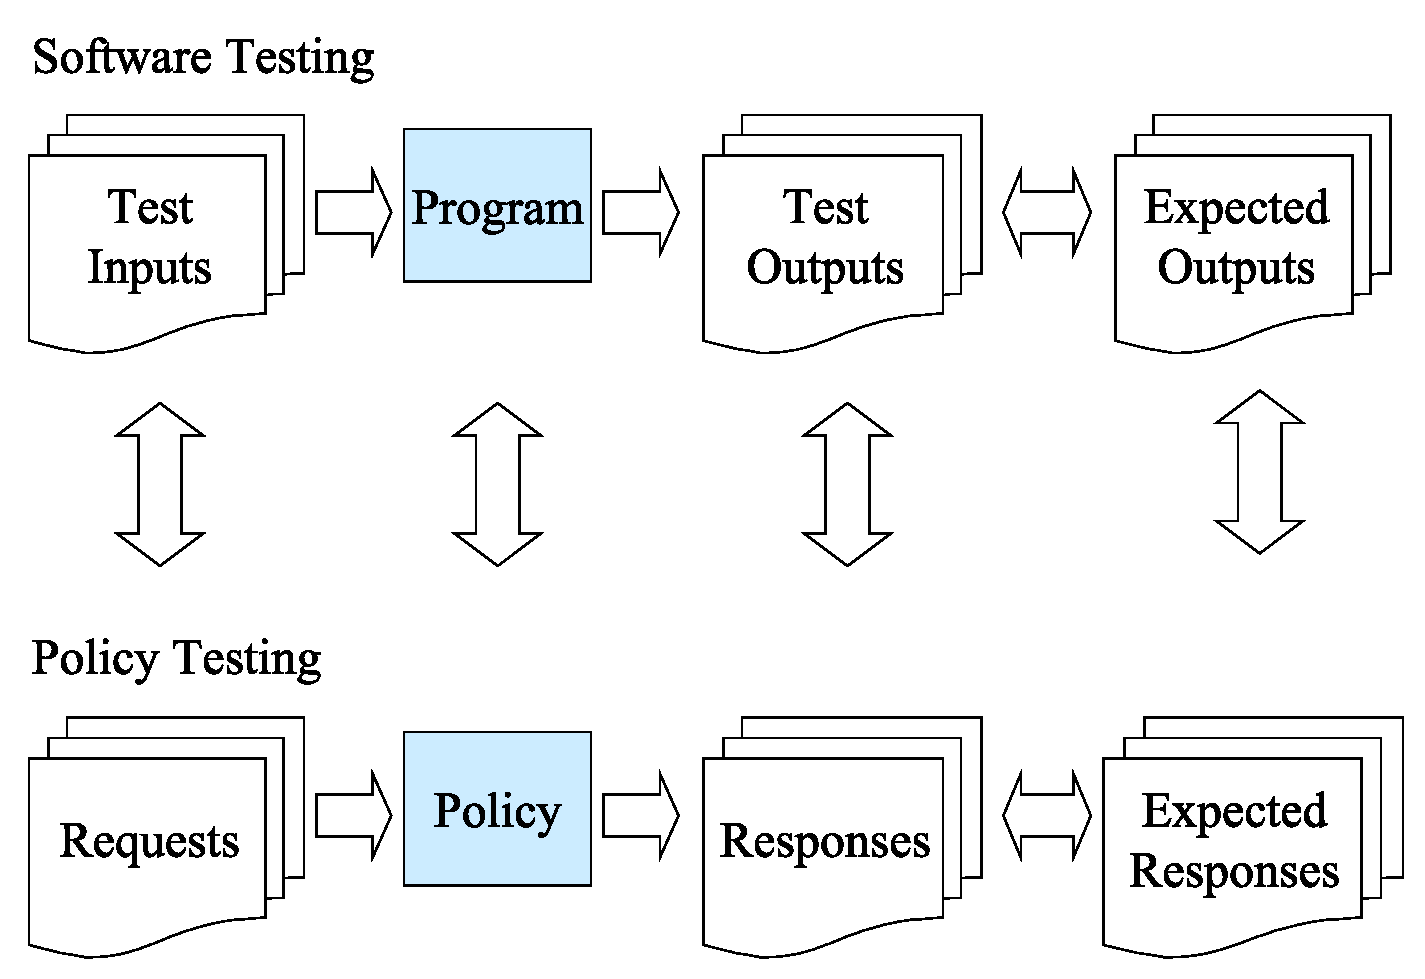
\includegraphics[width=3.25in]{policy-test}
    \caption{\label{fig:policy-test}Analogy between traditional software testing and policy testing.}
\end{figure}
